
\begin{figure}
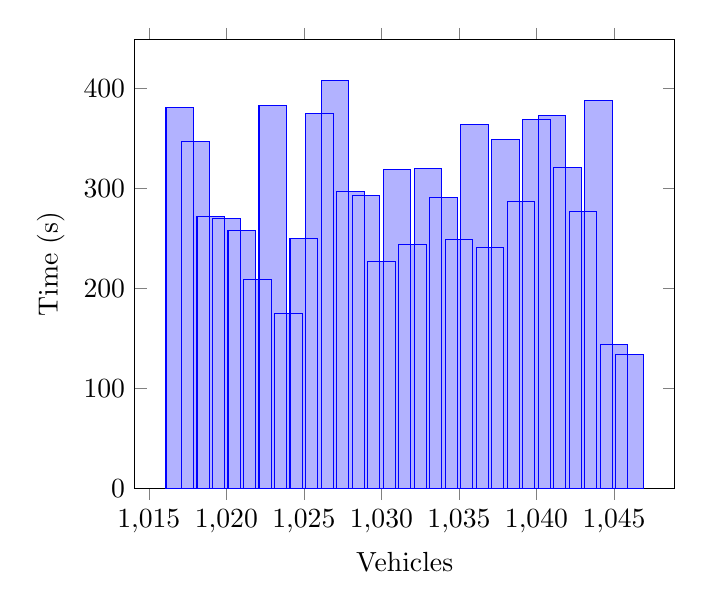
\begin{tikzpicture}
\begin{axis}[
legend style={anchor=west},
xlabel=Vehicles,
ylabel=Time (s),
ymin=0,
ybar,
]
\addplot coordinates {
(1041, 373)
(1021, 258)
(1019, 272)
(1026, 375)
(1022, 209)
(1020, 270)
(1023, 383)
(1034, 291)
(1045, 144)
(1042, 321)
(1035, 249)
(1028, 297)
(1031, 319)
(1046, 134)
(1036, 364)
(1017, 381)
(1024, 175)
(1043, 277)
(1037, 241)
(1039, 287)
(1029, 293)
(1033, 320)
(1025, 250)
(1038, 349)
(1027, 408)
(1018, 347)
(1040, 369)
(1030, 227)
(1032, 244)
(1044, 388)
};

\end{axis}
\end{tikzpicture}
\label{tik:time:100:96}
\caption{100 percent diving with GSC on route $96$}
\end{figure}
